\documentclass[hyperref=colorlinks]{beamer}
\mode<presentation>
\usetheme{iclpt}
\setbeamertemplate{navigation symbols}{}
\setbeamertemplate{headline}{
  \begin{beamercolorbox}[leftskip=.2cm,rightskip=.2cm,topskip=.2cm,ht=1.1cm,dp=0.1cm,wd=\textwidth]{institute in head/foot}
    \includegraphics[height=1cm]{icl.pdf}
    \hfill
%    \includegraphics[height=1cm]{../Pics/ATLAS-Logo-Square-Blue-RGB.png}
%    \includegraphics[height=1cm]{../Pics/CMS-Color.pdf}
    \includegraphics[height=1cm]{TalkPics/t2k_logo_large.png}

%??put t2k logo here
  \end{beamercolorbox}
}
\setbeamertemplate{footline}{
  \begin{beamercolorbox}[ht=.35cm,dp=0.2cm,wd=\textwidth,leftskip=.3cm]{author in head/foot}%
    \begin{minipage}[c]{5cm}%
      \usebeamerfont{author in head/foot}
      \insertshortauthor 
      \insertshorttitle
    \end{minipage}\hfill%
    \hfill
    \insertframenumber{} / \ref{lastframe}
    %\hfill
    \begin{minipage}{6cm}
      \hfill
      %\insertshorttitle
    \end{minipage}
  \end{beamercolorbox}%
}

\definecolor{beamer@icdarkblue}{RGB}{0,51,102}
\definecolor{beamer@icmiddleblue}{RGB}{0,82,150} 
\definecolor{beamer@iclightblue}{RGB}{200,212,232}
\definecolor{beamer@icmiddlered}{RGB}{204,51,0}
\definecolor{beamer@iclightred}{RGB}{232,212,32}

\usepackage{tikz}
\usetikzlibrary{arrows,shapes,backgrounds}
\usepackage{color}
\usepackage{tabularx,colortbl}
\usepackage{graphicx}
\usepackage{pdfpages}
\usepackage{feynmp}
\usepackage{rotating}
\usepackage{moresize}
\usepackage{slashed}
\usepackage{xcolor,colortbl}
\DeclareGraphicsRule{*}{mps}{*}{}
\hypersetup{colorlinks=false}

\title[Asimov comparisons with different dcp values]{\vspace{-0.2cm} Asimov comparisons with different dcp values}
\author[P. Dunne]{Patrick Dunne - Imperial College London}
\titlegraphic{
  \vspace{-0.4cm}
}
\date{}
\begin{document}
\tikzstyle{every picture}+=[remember picture]
\tikzstyle{na} = [baseline=-.5ex]
\begin{fmffile}{t2ktemplatefeyndiags}


  %TITLE PAGE
  %20 mins + 5 questions
  \section{Title}
  \begin{frame}
    \titlepage
  \end{frame}

  \begin{frame}
    \frametitle{Overview}
    \begin{block}{}
      \begin{itemize}
      \item Asked to study three new Asimov points by OA
      \item All based on point 1/A but with different values of dcp (see below)
      \item Energy spectra and Asimov contours with and without RC generated for each point
      \item All plots shown below marginalise over the two mass hierarchies
      \end{itemize}
      \centering
      \begin{tabular}{|l|c|c|c|c|}
        \hline
        Set & A & C & D & E \\
        \hline
        \hline
        $\sin^2(\theta_{12})$ & \multicolumn{4}{c|}{0.304}\\
        \hline
        $\sin^2(\theta_{13})$ & \multicolumn{4}{c|}{0.0217}\\
        \hline
        $\sin^2(\theta_{23})$ & \multicolumn{4}{c|}{0.528}\\
        \hline
        $\Delta m^2_{12}$ & \multicolumn{4}{c|}{7.35e-05}\\
        \hline
        $\Delta m^2_{23}$ & \multicolumn{4}{c|}{0.002509}\\
        \hline
        $\delta_{CP}$ & -1.601 & 0 & $\pi$ & $\frac{\pi}{2}$ \\
        \hline
      \end{tabular}
    \end{block}
  \end{frame}

  \begin{frame}
    \centering
    \huge\textcolor{beamer@icmiddleblue}{Energy Spectra}
  \end{frame}

  \begin{frame}
    \frametitle{Energy spectra - Asimov C ($\delta_{CP}=0$)}
    \centering
    \textcolor{red}{unoscillated} 

    \textcolor{blue}{oscillated}
    \includegraphics[width=\textwidth]{TalkPics/newasimovs_060916/plots_asimov1_dcp0/nominal_spectra.pdf}
  \end{frame}

  \begin{frame}
    \frametitle{Energy spectra - Asimov D ($\delta_{CP}=\pi$)}
    \centering
    \textcolor{red}{unoscillated} 

    \textcolor{blue}{oscillated}
    \includegraphics[width=\textwidth]{TalkPics/newasimovs_060916/plots_asimov1_dcppi/nominal_spectra.pdf}
  \end{frame}

  \begin{frame}
    \frametitle{Energy spectra - CP conserving (C and D)}
    \centering
    \textcolor{red}{unoscillated} 

    \textcolor{blue}{oscillated $\delta_{CP}=0$}

    \textcolor{cyan}{oscillated $\delta_{CP}=\pi$}

    \includegraphics[width=.4\textwidth]{TalkPics/newasimovs_060916/cpconservingspectraoverlay.png}
  \end{frame}


  \begin{frame}
    \frametitle{Energy spectra - Asimov A ($\delta_{CP}=-1.601$)}
    \centering
    \textcolor{red}{unoscillated} 

    \textcolor{blue}{oscillated}
    \includegraphics[width=\textwidth]{TalkPics/newasimovs_060916/plots_asimov1_dcpminus1601/nominal_spectra.pdf}
  \end{frame}


  \begin{frame}
    \frametitle{Energy spectra - Asimov E ($\delta_{CP}=\frac{\pi}{2}$)}
    \centering
    \textcolor{red}{unoscillated} 

    \textcolor{blue}{oscillated}
    \includegraphics[width=\textwidth]{TalkPics/newasimovs_060916/plots_asimov1_dcppiby2/nominal_spectra.pdf}
  \end{frame}

  \begin{frame}
    \centering
    \huge\textcolor{beamer@icmiddleblue}{woRC contours}
  \end{frame}

  \begin{frame}
    \frametitle{CP conserving sets - woRC appearance parameters}
    \centering
    \includegraphics[width=.65\textwidth]{TalkPics/newasimovs_060916/contours_newasimovcomparisons_woRC_060916/comparedcontours_th13dcp_cpconservingasimovs_official.pdf}
  \end{frame}

  \begin{frame}
    \frametitle{CP conserving sets - woRC disappearance parameters}
    \centering
    \includegraphics[width=.65\textwidth]{TalkPics/newasimovs_060916/contours_newasimovcomparisons_woRC_060916/comparedcontours_th23dm23_cpconservingasimovs_official.pdf}
  \end{frame}

  \begin{frame}
    \frametitle{CP conserving sets - woRC dcp}
    \centering
    \includegraphics[width=.65\textwidth]{TalkPics/newasimovs_060916/contours_newasimovcomparisons_woRC_060916/contours_1D_dcp_cpconservingasimovs_compare_official.pdf}
  \end{frame}

  \begin{frame}
    \frametitle{CP violating sets - woRC appearance parameters}
    \centering
    \includegraphics[width=.65\textwidth]{TalkPics/newasimovs_060916/contours_newasimovcomparisons_woRC_060916/comparedcontours_th13dcp_cpviolatingasimovs_official.pdf}
  \end{frame}

  \begin{frame}
    \frametitle{CP violating sets - woRC disappearance parameters}
    \begin{block}{}
      \begin{itemize}
      \item Differences seen here seem to be due to $\delta_{CP}=\pi$ fit choosing wrong mass hierarchy
      \item[-] Confirmed in contours where only one hierarchy is considered where differences are smaller (see backup) 
      \end{itemize}
    \end{block}
    \centering
    \includegraphics[width=.65\textwidth]{TalkPics/newasimovs_060916/contours_newasimovcomparisons_woRC_060916/comparedcontours_th23dm23_cpviolatingasimovs_official.pdf}
  \end{frame}

  \begin{frame}
    \frametitle{CP violating sets - woRC dcp}
    \centering
    \includegraphics[width=.65\textwidth]{TalkPics/newasimovs_060916/contours_newasimovcomparisons_woRC_060916/contours_1D_dcp_cpviolatingasimovs_compare_official.pdf}
  \end{frame}

  \begin{frame}
    \centering
    \huge\textcolor{beamer@icmiddleblue}{wRC contours}
  \end{frame}


  \begin{frame}
    \frametitle{CP conserving sets - wRC appearance parameters}
    \centering
    \includegraphics[width=.65\textwidth]{TalkPics/newasimovs_060916/contours_newasimovcomparisons_wRC_060916/comparedcontours_th13dcp_cpconservingasimovs_official.pdf}
  \end{frame}

  \begin{frame}
    \frametitle{CP conserving sets - wRC disappearance parameters}
    \centering
    \includegraphics[width=.65\textwidth]{TalkPics/newasimovs_060916/contours_newasimovcomparisons_wRC_060916/comparedcontours_th23dm23_cpconservingasimovs_official.pdf}
  \end{frame}

  \begin{frame}
    \frametitle{CP conserving sets - wRC dcp}
    \centering
    \includegraphics[width=.65\textwidth]{TalkPics/newasimovs_060916/contours_newasimovcomparisons_wRC_060916/contours_1D_dcp_cpconservingasimovs_compare_official.pdf}
  \end{frame}

  \begin{frame}
    \frametitle{CP violating sets - wRC appearance parameters}
    \centering
    \includegraphics[width=.65\textwidth]{TalkPics/newasimovs_060916/contours_newasimovcomparisons_wRC_060916/comparedcontours_th13dcp_cpviolatingasimovs_official.pdf}
  \end{frame}

  \begin{frame}
    \frametitle{CP violating sets - wRC disappearance parameters}
    \centering
    \includegraphics[width=.65\textwidth]{TalkPics/newasimovs_060916/contours_newasimovcomparisons_wRC_060916/comparedcontours_th23dm23_cpviolatingasimovs_official.pdf}
  \end{frame}

  \begin{frame}
    \frametitle{CP violating sets - wRC dcp}
    \centering
    \includegraphics[width=.65\textwidth]{TalkPics/newasimovs_060916/contours_newasimovcomparisons_wRC_060916/contours_1D_dcp_cpviolatingasimovs_compare_official.pdf}
  \end{frame}



  \begin{frame}
    \frametitle{}
    \label{lastframe}
    \begin{block}{}
      \begin{itemize}
      \item Little difference between CP conserving asimovs
      \item[-] Spectra are very similar (see right
      \item CP violating Asimovs show tighter exclusions for -1.601 than $\frac{\pi}{2}$
      \item[-] This is due to there being a lot more $\nu_{e}$ events for -1.601 than for $\frac{\pi}{2}$
      \item wRC being processed now
      \end{itemize}
    \end{block}
  \end{frame}

  %Backup goes here
  \begin{frame}
    \centering
    \huge\textcolor{beamer@icmiddleblue}{Backup}
  \end{frame}

  \begin{frame}
    \frametitle{CP violating sets - woRC disappearance parameters NH \& IH separately}
    \centering
    \includegraphics[width=.5\textwidth]{TalkPics/newasimovs_060916/contours_newasimovcomparisons_woRC_060916/comparedcontours_th23dm23_cpviolatingasimovs_NH_official.pdf}
    \includegraphics[width=.5\textwidth]{TalkPics/newasimovs_060916/contours_newasimovcomparisons_woRC_060916/comparedcontours_th23dm23_cpviolatingasimovs_IH_official.pdf}
  \end{frame}
  
\end{fmffile}
\end{document}

